\documentclass[tikz,border=2mm]{standalone}
\usepackage[T1]{fontenc}
\usepackage{lmodern}
\usetikzlibrary{arrows.meta, shapes.geometric, positioning, fit, backgrounds}

\begin{document}
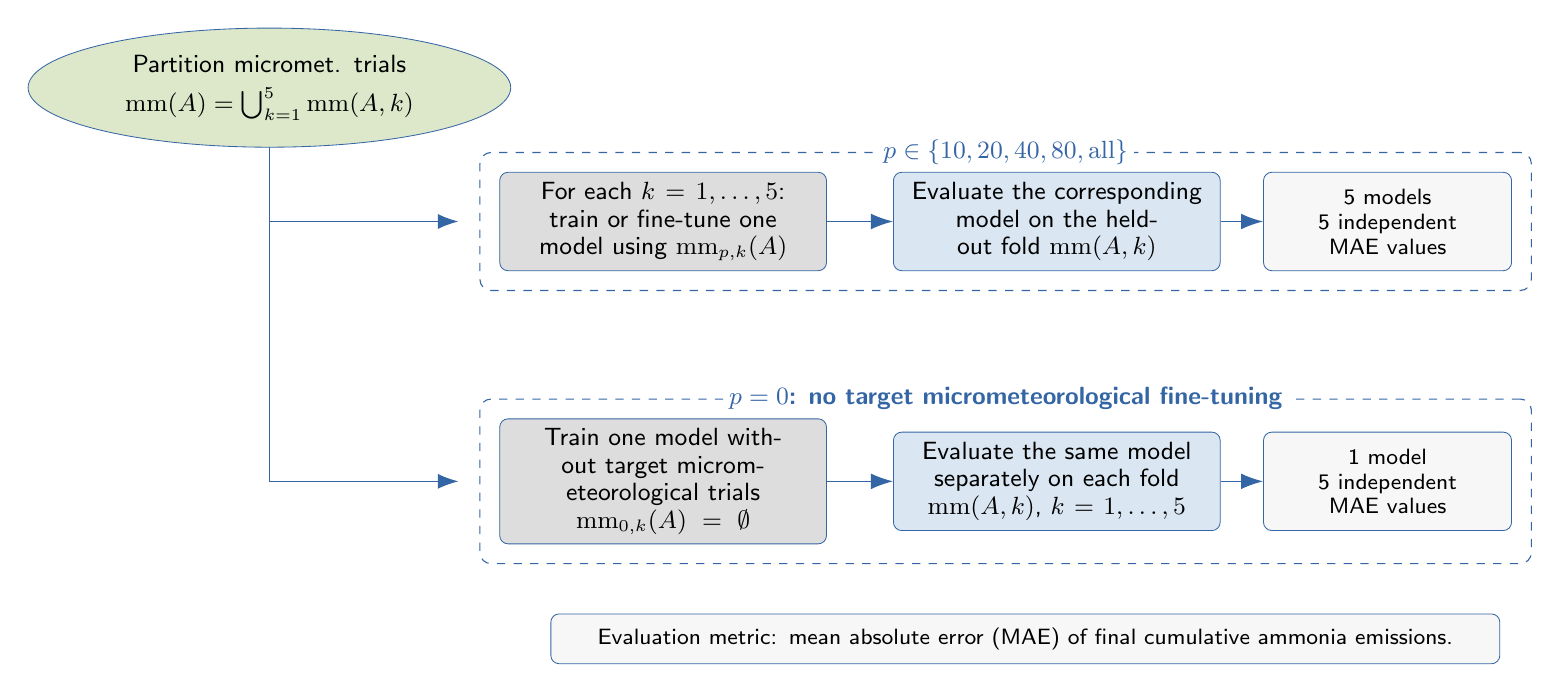
\begin{tikzpicture}[
  font=\sffamily,
  >=Latex,
  blueLine/.style={draw=blueLine},
  source/.style={ellipse, blueLine, fill=dataFill, line width=0.3pt,
                 minimum width=4.5cm, minimum height=1.30cm,
                 align=center, text width=4.10cm,
                 font=\sffamily\fontsize{9}{10}\selectfont},
  process/.style={rounded corners=3pt, blueLine, fill=modelFill, line width=0.3pt,
                  minimum width=4.15cm, minimum height=1.25cm,
                  align=center, text width=3.7cm,
                  font=\sffamily\fontsize{9}{10}\selectfont},
  eval/.style={rounded corners=3pt, blueLine, fill=evalFill, line width=0.3pt,
               minimum width=4.15cm, minimum height=1.25cm,
               align=center, text width=3.7cm,
               font=\sffamily\fontsize{9}{10}\selectfont},
  result/.style={rounded corners=3pt, blueLine, fill=noteFill, line width=0.3pt,
                 minimum width=3.15cm, minimum height=1.25cm,
                 align=center, text width=2.75cm,
                 font=\sffamily\fontsize{8}{9}\selectfont},
  lane/.style={rounded corners=4pt, blueLine, dashed, line width=0.4pt,
               inner sep=7pt},
  lanehead/.style={font=\sffamily\fontsize{9}{10}\selectfont\bfseries,
                   align=center, text=blueLine},
  note/.style={rounded corners=3pt, blueLine, fill=noteFill, line width=0.3pt,
               align=center, text width=11.7cm, inner sep=5pt,
               font=\sffamily\fontsize{8}{9}\selectfont},
  arrow/.style={blueLine, line width=0.45pt, -{Latex[length=2.8mm,width=2mm]}},
  branch/.style={blueLine, line width=0.4pt, -{Latex[length=2.6mm,width=1.9mm]}}
]

\definecolor{blueLine}{RGB}{52,101,164}
\definecolor{dataFill}{RGB}{221,232,203}
\definecolor{modelFill}{RGB}{221,221,221}
\definecolor{evalFill}{RGB}{218,230,242}
\definecolor{noteFill}{RGB}{247,247,247}

\node[source] (partition) at (0,0) {Partition micromet. trials\\[1.5mm]\mbox{$\mathrm{mm}(A)=\bigcup_{k=1}^{5}\mathrm{mm}(A,k)$}};

% Models that use target micrometeorological trials
\node[process] (trainp) at (5.0,-1.7) {For each $k=1,\ldots,5$:\\train or fine-tune one model using $\mathrm{mm}_{p,k}(A)$};
\node[eval] (evalp) at (10.0,-1.7) {Evaluate the corresponding model on the held-out fold $\mathrm{mm}(A,k)$};
\node[result] (resp) at (14.2,-1.7) {5 models\\5 independent MAE values};
\node[lane, fit=(trainp)(evalp)(resp)] (lanep) {};
\node[lanehead, fill=white, inner sep=2pt] at (lanep.north) {$p\in\{10,20,40,80,\mathrm{all}\}$};

% Models that do not use target micrometeorological trials
\node[process] (train0) at (5.0,-5.0) {Train one model without target micrometeorological trials\\$\mathrm{mm}_{0,k}(A)=\emptyset$};
\node[eval] (eval0) at (10.0,-5.0) {Evaluate the same model separately on each fold $\mathrm{mm}(A,k)$, $k=1,\ldots,5$};
\node[result] (res0) at (14.2,-5.0) {1 model\\5 independent MAE values};
\node[lane, fit=(train0)(eval0)(res0)] (lane0) {};
\node[lanehead, fill=white, inner sep=2pt] at (lane0.north) {$p=0$: no target micrometeorological fine-tuning};

\begin{scope}[on background layer]
  \draw[blueLine, line width=0.4pt] (partition.center) -- (0,-0.85);
  \draw[branch] (0,-0.85) |- (2.4,-1.7);
  \draw[branch] (0,-0.85) |- (2.4,-5.0);
\end{scope}
\draw[arrow] (trainp) -- (evalp);
\draw[arrow] (evalp) -- (resp);
\draw[arrow] (train0) -- (eval0);
\draw[arrow] (eval0) -- (res0);

\node[note] at (9.6,-7.0) {Evaluation metric: mean absolute error (MAE) of final cumulative ammonia emissions.};

\end{tikzpicture}
\end{document}
